\section{Virtuoso}
\label{sec:virtuoso}

Virtuoso Universal Server,\footnote{\url{https://virtuoso.openlinksw.com/}} often called just Virtuoso, or OpenLink Virtuoso, at core is a high-performance object-relational \acs{SQL} database. It was born in 1998 when OpenLink Software wanted to merge in a single solution its Universal Data Access Middleware and Kubl \acs{DBMS}.\footnote{\url{https://vos.openlinksw.com/owiki/wiki/VOS/VOSHistory}}

Besides the database, Virtuoso has a built-in web server with support to Virtuoso's Web Language (VSP), and the most popular scripting languages such as PHP or ASP.NET. This same web server provides SOAP and REST access to Virtuoso stored procedures, supporting a broad set of WS* protocols.
Virtuoso has also a built-in WebDAV repository to host static and dynamic web content and provide versioning, making it a convenient and secure place for keeping files on the net.\footnote{\url{https://vos.openlinksw.com/owiki/wiki/VOS/VOSIntro}}

Since 2005, Virtuoso supports \ac{SPARQL} for querying \ac{RDF} data stored in its Quad Store database. In particular, it supports the \ac{HTTP}-based \ac{SPARQL} Protocol, \ac{SPARQL} federated queries, different exchange formats such as \acs{HTML}, \ac{CSV}, \ac{TSV}, \ac{JSON}, \ac{RDF}/\ac{XML}, Turtle, N-Triples, and more. For this reasons Virtuoso has become the most popular and efficient tool for serving a \ac{SPARQL} endpoint, which is usually located at \verb#http://{host}/sparql#. Figure \ref{fig:virtuoso-sparql} shows an example of how the endpoint looks like.

\begin{figure}[!ht]
  \centering
  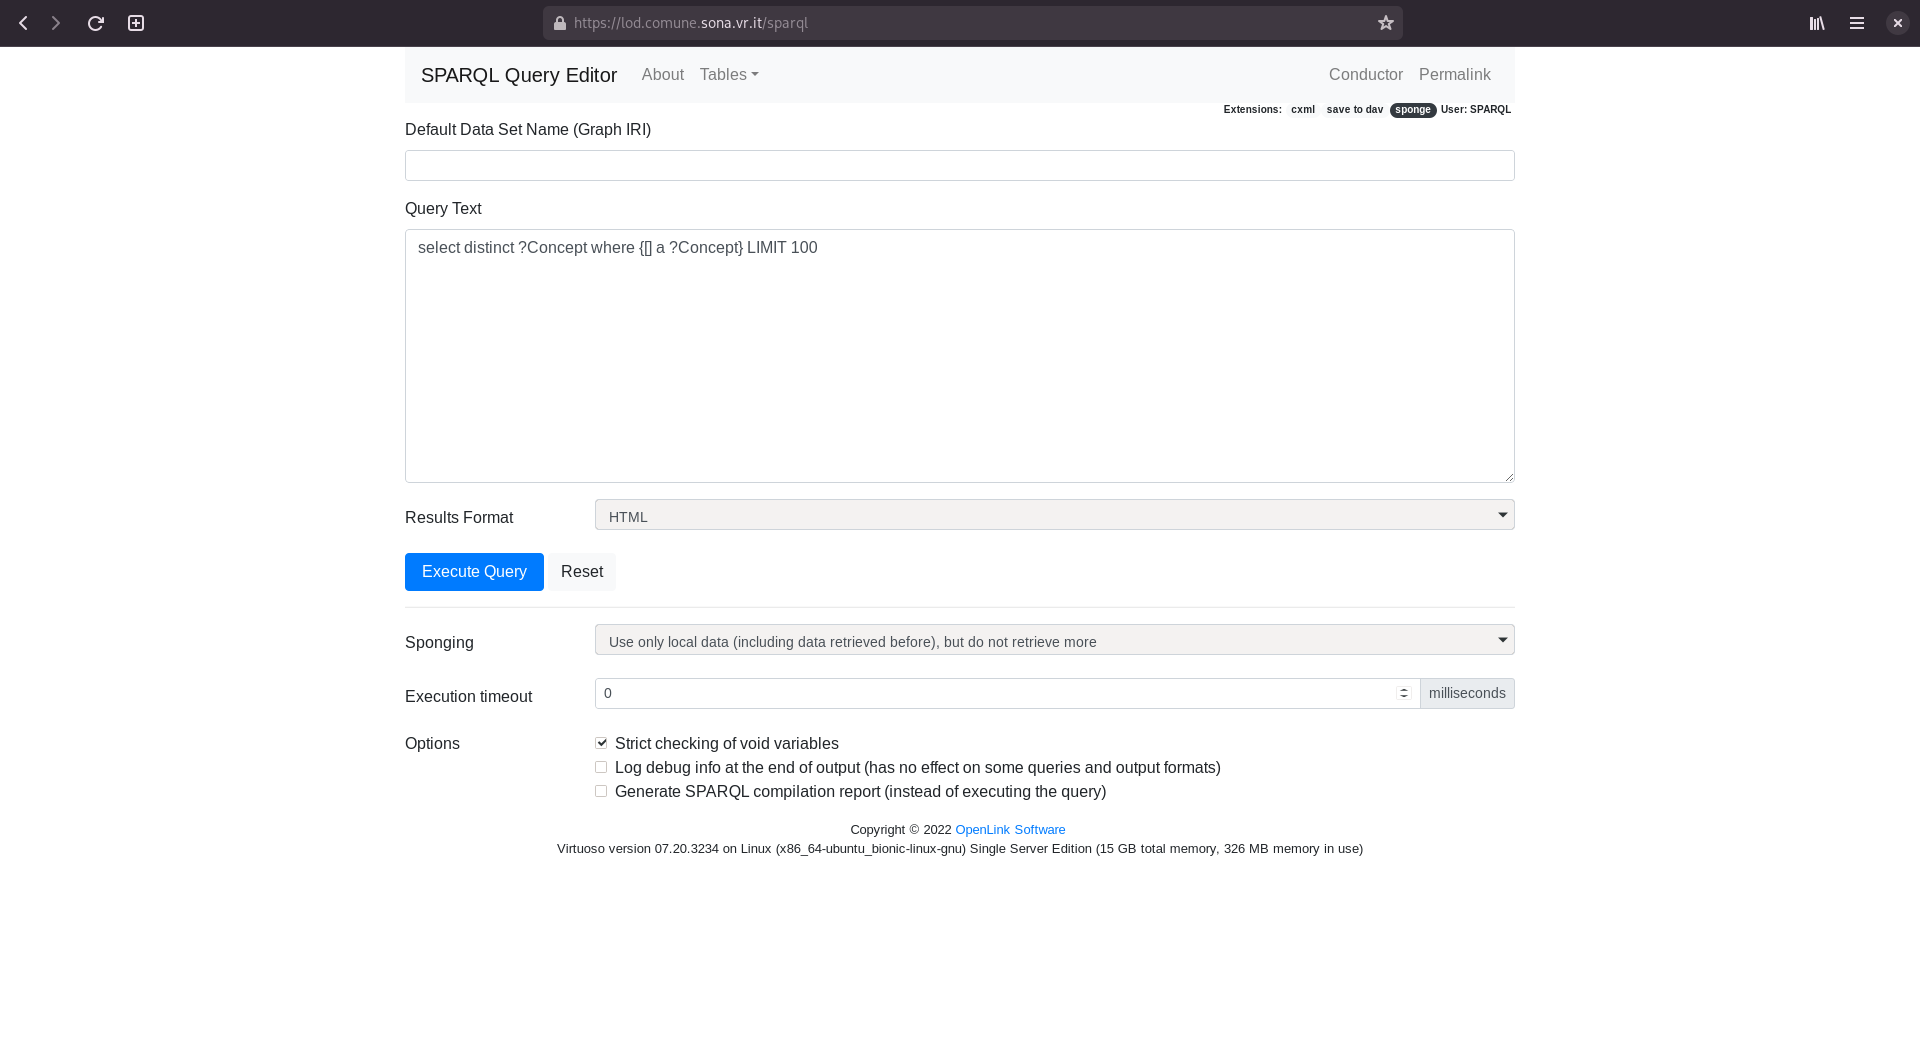
\includegraphics[width=\columnwidth]{images/virtuoso/virtuoso-sparql}
  \caption{A snapshot of the Virtuoso \ac{SPARQL} endpoint.}
  \label{fig:virtuoso-sparql}
\end{figure}

All the aspects of a Virtuoso instance can be managed through the Virtuoso Conductor, that is located at \verb#http://{host}/conductor#. For example, from "Linked Data" tab it is possible to add and remove \ac{RDF} graphs, import schemas, declare persistent namespaces, generate statistics such as the number of classes, triples, subjects, \etc.

There are many methods to insert an \ac{RDF} resource into the Virtuoso Quad Store. Some of them are:

\begin{description}
  \item[Virtuoso Conductor] Using Virtuoso Conductor web interface, under "Linked Data" and then "Quad Store Upload" tab it is possible to upload a \ac{RDF} resource directly into the Virtuoso Quad Store. It is also possible to assign a graph \ac{IRI} where to upload the resource. A snapshot of this feature is shown in Figure \ref{fig:virtuoso-upload}.
  \begin{figure}[!ht]
    \centering
    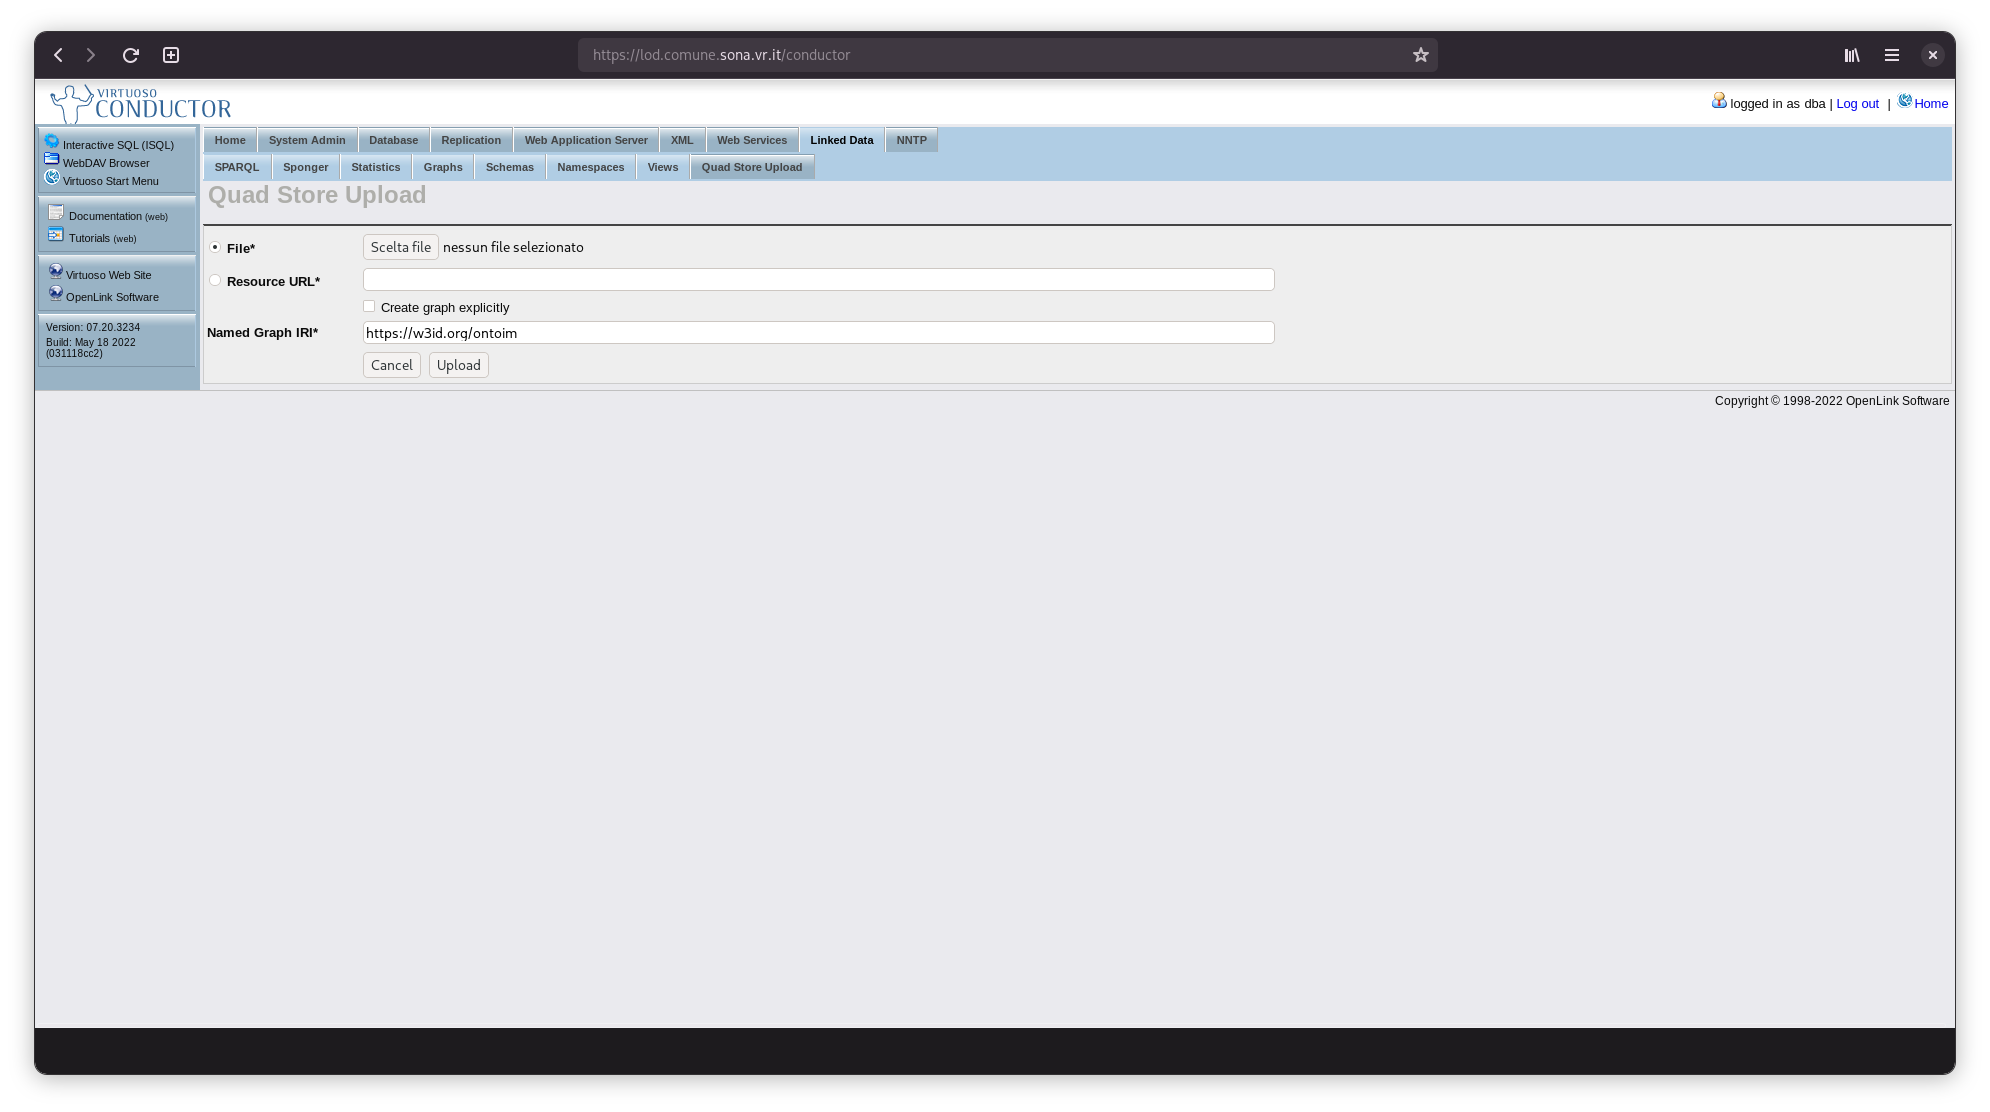
\includegraphics[width=\columnwidth]{images/virtuoso/virtuoso-upload}
    \caption{A snapshot of the "Quad Store Upload" tab.}
    \label{fig:virtuoso-upload}
  \end{figure}

  \item[RDF Sink Folder] WebDAV supports a special folder called \verb#rdf_sink#. This folder can be used to upload \ac{RDF} files from any WebDAV client, which are automatically uploaded to the Virtuoso Quad Store.

  \item[\ac{HTTP} PUT] \ac{RDF} files can be uploaded to a \verb#rdf_sink# folder through the \ac{HTTP} PUT method. An example using cURL can be:
  \begin{verbatim}
    curl -T foaf.rdf
      http://localhost:8890/DAV/home/dba/rdf_sink/foaf.rdf
      -u dba:dba
  \end{verbatim}

  \item[\ac{HTTP} POST] Virtuoso supports \ac{HTTP} POST method to execute \ac{SPARQL}/Update language using \verb#Content-Type: application/sparql-query# in the \ac{HTTP} request headers. An example using cURL can be:
  \begin{verbatim}
    curl -i -d "INSERT {
      <http://w3id.org/people/lucamartinelli>
      <http://www.w3.org/1999/02/22-rdf-syntax-ns#type>
      <http://xmlns.com/foaf/0.1/User>
    }" -u "dba:dba"
    -H "Content-Type: application/sparql-query"
    http://localhost:8890/DAV/home/xx/yy
  \end{verbatim}

  \item[\ac{SPARQL} endpoint] If the user has the permission to insert graphs directly from the \ac{SPARQL} endpoint, using the \ac{SPARQL}/Update language, as in the example above.
\end{description}

These were just some features provided by Virtuoso Universal Server in order to use it as a \ac{SPARQL} endpoint and \ac{RDF} data store system. The full documentation on how to use Virtuoso is available at \url{https://vos.openlinksw.com/owiki/wiki/VOS}.